\documentclass[12pt]{article}
\usepackage{geometry}
\usepackage{graphicx}
\usepackage{float}
\usepackage{caption}
\usepackage{subcaption}
\usepackage{booktabs}
\usepackage{amsmath}
\usepackage{hyperref}
\usepackage{siunitx}
\usepackage{tocloft}
\renewcommand{\cftsecfont}{\normalsize} % font size for sections
\renewcommand{\cftsubsecfont}{\small}   % smaller font for subsections
\renewcommand{\cftsecpagefont}{\normalsize} 
\renewcommand{\cftsubsecpagefont}{\small}
\renewcommand{\cftbeforesecskip}{0pt}   % remove extra vertical space
\renewcommand{\cftbeforesubsecskip}{0pt}
\setlength{\cftsecindent}{0pt}
\setlength{\cftsubsecindent}{15pt}

\geometry{margin=1in}
\graphicspath{{figures/}}

\begin{document}

% ------------------ COVER PAGE ------------------
\begin{titlepage}
    \centering
    \vspace*{0.1cm}
    {\huge LUT Characterization \\[0.5em]}
    {\large Fall 2025 \\[2em]}

    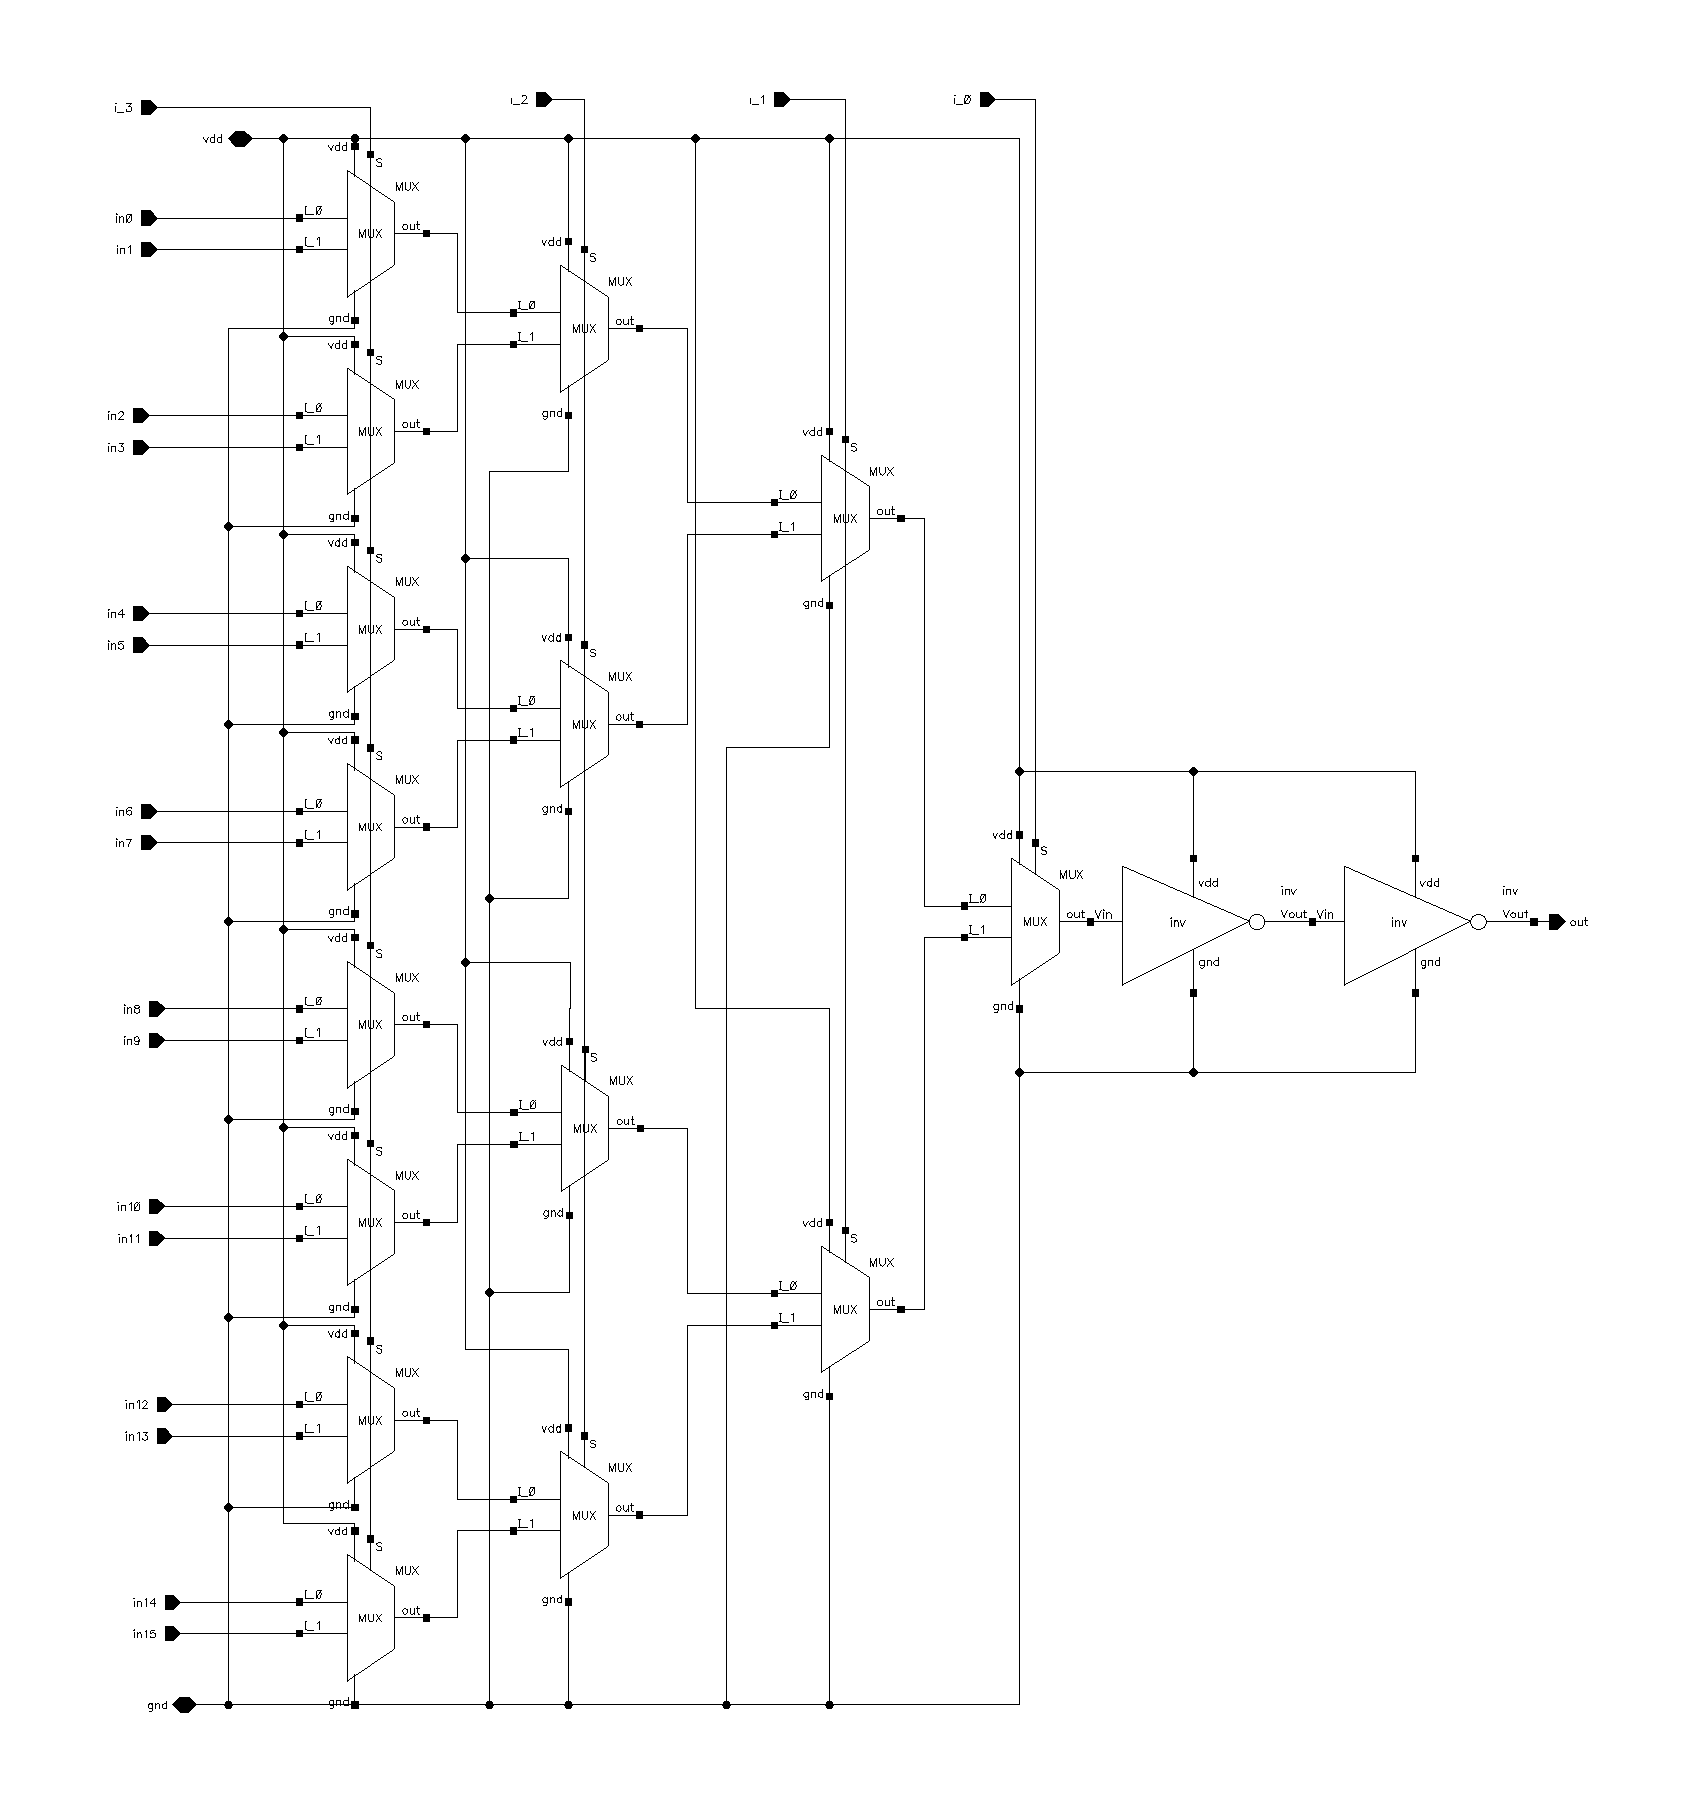
\includegraphics[width=\linewidth]{LUT_sch.png}\\[2em]

    \textbf{Authors:} Krishna Karthikeya Chemudupati, Taarana Jammula \\[2em]

    \vfill
\end{titlepage}

% ------------------ TABLE OF CONTENTS ------------------
\tableofcontents
\newpage

% ------------------ SECTION 1 ------------------
\section{Baseline Design Schematics}

\subsection{Minimum Size Inverter}

\subsubsection*{Schematic}



\subsubsection*{Symbol}



\newpage

\subsection{2:1 MUX Design}



\newpage

\subsection{16:1 LUT Design}



\newpage

% ------------------ SECTION 2 ------------------
\section{Baseline Design Validation and Logical Test}
\subsection{Test Schematic and Case}



\newpage

\subsection{Simulation Results}



\newpage

% ------------------ SECTION 3 ------------------
\section{Baseline Delay Measurement}
\subsection{Test Schematic}



\newpage

\subsection{Test Case}



\newpage

\subsection{Simulation Results and Metric Value}



\newpage

% ------------------ SECTION 4 ------------------
\section{Baseline Frequency Measurement}
\subsection{Test Schematic}



\newpage

\subsection{Simulation Results and Metric Value}





\begin{figure}[H]
    \centering
    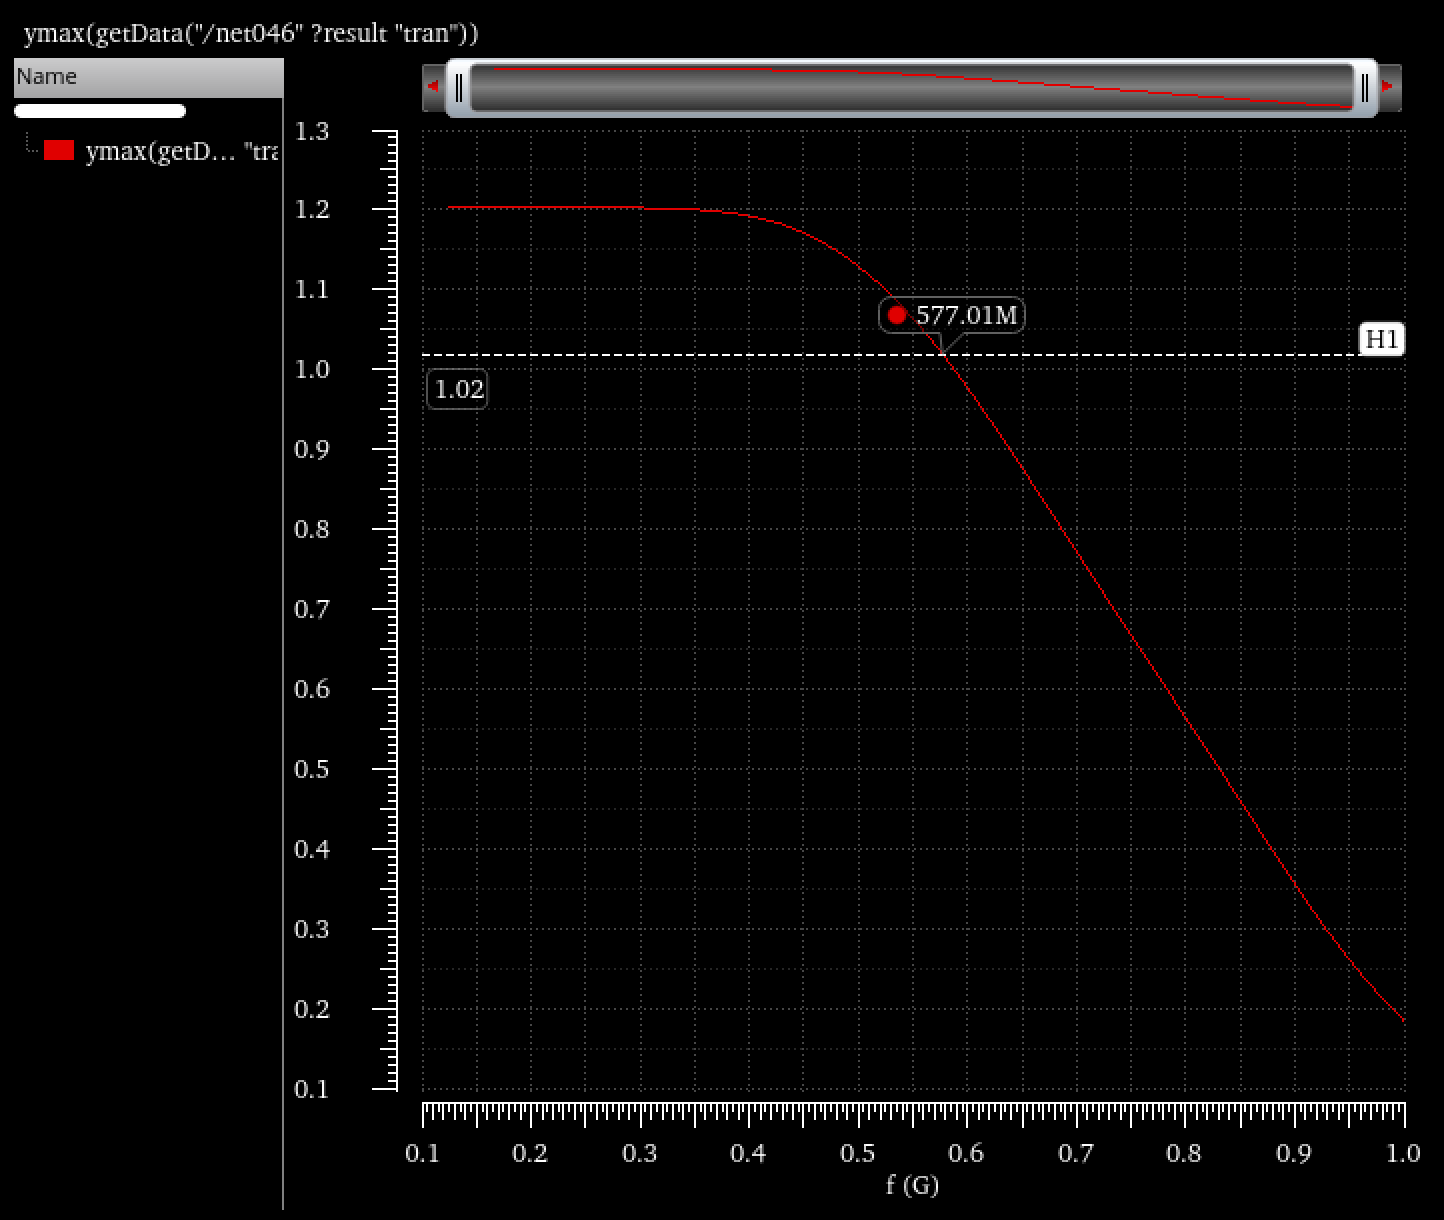
\includegraphics[width=0.75\linewidth]{writeup//figures/max_frequencies.png}
    \caption{Extracting frequency value that allows for 85\% of VDD after buffer stage}
\end{figure}

\newpage

% ------------------ SECTION 5 ------------------
\section{Baseline Energy Measurement}
\subsection{Test Schematic}



\newpage

\subsection{Test Case}



\newpage

\subsection{Simulation Results and Metric Value}



\newpage

% ------------------ SECTION 6 ------------------
\section{Optimized Design}
\subsection{Optimized Design Schematics}



\newpage

\subsection{Optimization Process}



\newpage

% ------------------ SECTION 7 ------------------
\section{Optimized Design Validation and Logical Test}
\subsection{Test Schematic and Case}



\newpage

\subsection{Simulation Results}



\newpage

% ------------------ SECTION 8 ------------------
\section{Optimized Delay Measurement}
\subsection{Test Schematic}



\newpage

\subsection{Test Case}



\newpage

\subsection{Simulation Results and Metric Value}



\newpage

% ------------------ SECTION 9 ------------------
\section{Optimized Frequency Measurement}
\subsection{Test Schematic}



\newpage

\subsection{Simulation Results and Metric Value}



\newpage

% ------------------ SECTION 10 ------------------
\section{Optimized Energy Measurement}
\subsection{Test Schematic}



\newpage

\subsection{Test Case}



\newpage

\subsection{Simulation Results and Metric Value}



\newpage

% ------------------ SECTION 11 ------------------
\section{Comparison Table}



\newpage

% ------------------ SECTION 12 ------------------
\section{Discussion and Conclusions}



\end{document}